\documentclass[12pt]{article}
\usepackage{natbib}
\usepackage{url}
\usepackage{fullpage}

\usepackage{times}

\usepackage{graphicx}
\usepackage{float}
\usepackage{capt-of}
\usepackage{subcaption}

\begin{document}
\title{Reflection Space Image Based Environment Mapping}
\author{Kyung yul Kevin Lim, Myron Liu}
\date{\today}
\maketitle

\section{Abstract}
We implement Reflection Space Image Based Rendering as described by Cabral et al.\cite{cabral1999reflection}. The goal is to generate a scene in which the user can rotate around the object lit by an HDR environment map, and observe view dependent BRDF changes in real time.

\section{Results}
\begin{figure}[H]
\centering
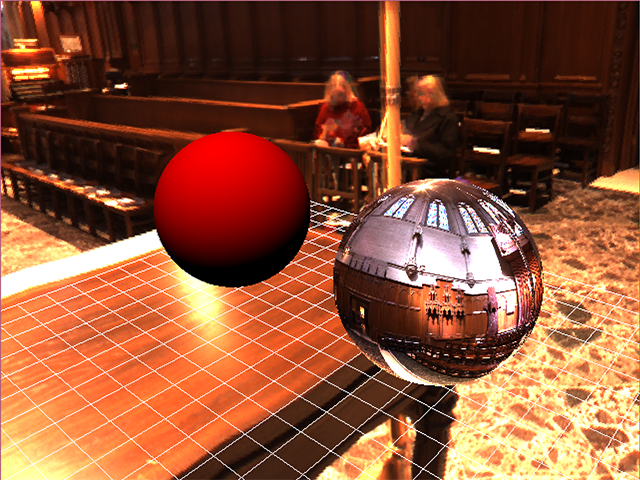
\includegraphics[width=0.75\textwidth]{{Figures/Milestone.png}}
\caption{A diffuse sphere and a fully mirrored sphere} 
\label{fig:milestone}
\end{figure}

\bibliographystyle{plain}
\bibliography{MilestoneReport}

\end{document}

